% ================================================================
% chapters/chapter4.tex --- RECONSTRUCTION (même structure que ch.3)
% ----------------------------------------------------------------
% Backlog restructuré~: Titre + Charge (j/h) ajoutées, Statut retiré
% + phrase de synthèse. Charge (j/h) = MES ESTIMATIONS RELATIVES,
% pas des mesures réelles --- à remplacer si tu as de vraies données.
% Rien d'autre n'est modifié dans ce chapitre.
% ================================================================

\chapter{Itération~2 --- Dashboards Web Admin et Company}

\section{Introduction}

Cette itération couvre le développement des deux interfaces web de \tynassit{}~:
le \textbf{dashboard Admin} destiné aux équipes Tynass, et le \textbf{dashboard Company}
destiné aux entreprises clientes. Les deux dashboards sont développés avec React,
TypeScript et déployés séparément sur Vercel pour garantir une isolation totale.

\section{Planification de l'itération~2}

\subsection{Objectifs}

\begin{itemize}
  \item Livrer 7 pages fonctionnelles pour le dashboard Admin.
  \item Livrer 6 pages fonctionnelles pour le dashboard Company.
  \item Connecter les deux dashboards au backend via l'API REST.
  \item Déployer les deux dashboards en production sur Vercel.
\end{itemize}

\subsection{Tâches et estimations de l'itération~2}

\begin{table}[H]
  \centering
  \small
  \setlength{\tabcolsep}{5pt}
  \begin{tabularx}{\textwidth}{cp{3.5cm}Xc>{\footnotesize}c}
    \toprule
    \textbf{ID} & \textbf{Titre} & \textbf{Tâches principales} & \textbf{MoSCoW} & \textbf{Charge estimée (j/h)} \\
    \midrule
    US-06 & Connexion Admin &
      LoginPage admin + AuthProvider + JWT localStorage & \must{} & 1,5 \\
    US-07 & KPIs du dashboard &
      DashboardPage --- 4 KPIs + Top 5 Companies/Trainings & \must{} & 2 \\
    US-08 & Gestion des entreprises &
      CompaniesPage --- CRUD + toggle + assign formations & \must{} & 2,5 \\
    US-09 & Gestion des casques &
      DevicesPage --- activation (code 6 chiffres) + révocation & \must{} & 2 \\
    US-10 & Filtrage des sessions &
      SessionsPage --- filtres company/training/date & \should{} & 1,5 \\
    US-11 & Connexion Company &
      LoginPage company + AuthProvider company & \must{} & 1 \\
    US-12 & Gestion des employés &
      EmployeesPage --- CRUD + accessCode + PIN & \must{} & 2 \\
    US-13 & Historique Company &
      SessionsPage company --- historique + pagination & \should{} & 1,5 \\
    \midrule
    \multicolumn{4}{r}{\textbf{Total estimé}} & \textbf{14} \\
    \bottomrule
  \end{tabularx}
  \caption{Tâches et estimations --- Itération~2}
  \label{tab:backlog_s2}
\end{table}

\noindent Toutes les user stories de cette itération ont été livrées.

\section{Conception de l'itération~2}

Cette section présente les choix technologiques retenus pour les deux dashboards web
ainsi que le système d'authentification mis en place.

\subsection{Décisions architecturales --- Frontend}

\begin{table}[H]
  \centering
  \begin{tabularx}{\textwidth}{lllX}
    \toprule
    \textbf{Composant} & \textbf{Retenu} & \textbf{Alternative} & \textbf{Justification} \\
    \midrule
    Framework  & React + TS  & Vue, Angular   & Maîtrise préalable, écosystème npm,
                                                typage strict \\
    Language   & TypeScript  & JavaScript     & Détection erreurs à la compilation,
                                                interfaces pour types API \\
    Bundler    & Vite        & CRA, Webpack   & Démarrage instantané (ESM natif),
                                                HMR ultra-rapide \\
    Router     & React Router v6 & TanStack Start & SSR bloquait les appels fetch API
                                                    côté client \\
    Data       & TanStack Query & SWR, Axios  & Cache automatique, invalidation après
                                                mutation, états loading/error natifs \\
    UI         & Shadcn UI   & Material UI    & Composants copiés dans le projet
                                                (pas de lock-in), basés sur Radix UI \\
    CSS        & Tailwind v3 & Tailwind v4    & Incompatibilité v4 avec composants
                                                Shadcn UI \\
    Animations & Framer Motion & CSS seul    & Transitions fluides, animations déclaratives \\
    Toasts     & Sonner      & React-Toastify & API simple, design moderne \\
    Déploiement & Vercel     & Netlify        & CI/CD automatique depuis GitHub \\
    \bottomrule
  \end{tabularx}
  \caption{Décisions architecturales --- Dashboards React}
  \label{tab:archi_frontend}
\end{table}

\subsection{Pourquoi deux projets séparés~?}

Un seul projet avec gestion des rôles aurait été possible, mais deux projets séparés
ont été préférés pour les raisons suivantes~:

\begin{itemize}
  \item \textbf{Isolation totale des données}~: le dashboard Company n'a accès qu'aux
    routes \texttt{/api/company/*}, jamais aux routes admin.
  \item \textbf{Déploiements indépendants}~: une mise à jour du dashboard Admin
    n'affecte pas le dashboard Company.
\end{itemize}

\subsection{Système d'authentification}

L'authentification aux dashboards repose sur un jeton JWT. La figure~\ref{fig:seq_login_admin}
présente la séquence de connexion d'un administrateur, depuis la saisie de ses identifiants
jusqu'à la validation du jeton et le chargement de son profil.

\begin{figure}[H]
  \centering
  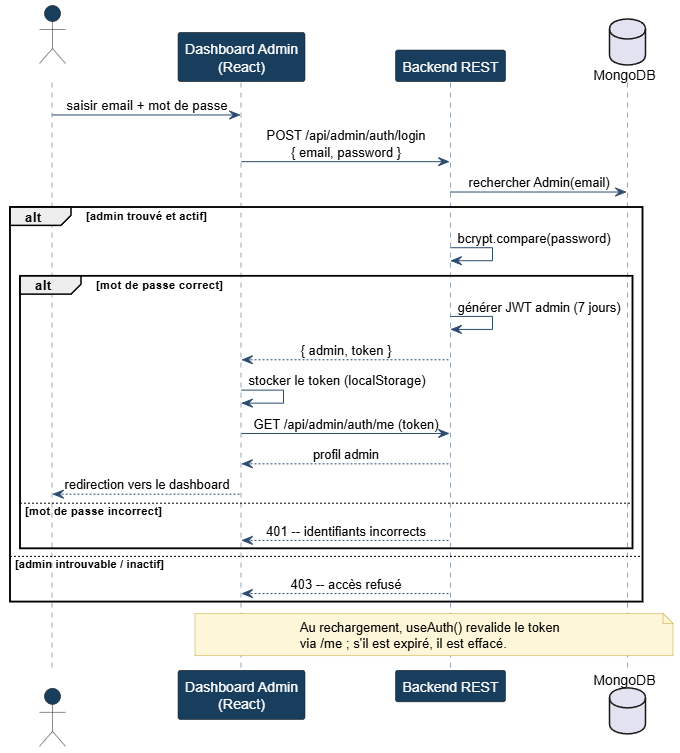
\includegraphics[width=0.9\textwidth]{../images/seqLoginAdmin.png}
  \caption{Diagramme de séquence --- login administrateur}
  \label{fig:seq_login_admin}
\end{figure}

Le JWT admin est stocké dans \texttt{localStorage("admin\_token")}. Au chargement de
l'application, le hook \texttt{useAuth()} appelle \texttt{api.getMe()} pour valider
le token et récupérer le profil admin. Si le token est expiré, \texttt{.catch()}
l'efface automatiquement et redirige vers la page de connexion.

\subsection{Cas d'utilisation --- Descriptions textuelles}

\begin{ucbox}{Activer un casque (côté Dashboard)}
  \begin{tabular}{lp{9cm}}
    \textbf{Pré-conditions} & Admin connecté, casque affichant un code 6 chiffres. \\
    \textbf{Acteur}         & Staff Admin Tynass. \\
    \textbf{Scénario}       &
      1. Admin ouvre DevicesPage et clique « Activate Device ». \newline
      2. Admin saisit le code 6 chiffres affiché sur le casque. \newline
      3. Admin sélectionne l'entreprise propriétaire du casque. \newline
      4. Admin saisit un label optionnel (ex~: « Salle de formation A »). \newline
      5. Dashboard appelle \texttt{POST /api/company/devices/activate}. \newline
      6. Succès~: le casque apparaît dans la liste comme « Active ». \\
    \textbf{Exceptions}     & Code expiré (15 min) → message d'erreur, régénérer. \\
    \textbf{Post-conditions}& Casque actif, apparaît dans la liste des devices. \\
  \end{tabular}
\end{ucbox}

\vspace{0.5cm}

\begin{ucbox}{Créer un employé avec accessCode et PIN}
  \begin{tabular}{lp{9cm}}
    \textbf{Pré-conditions} & Manager Company connecté au dashboard. \\
    \textbf{Acteur}         & Company (client B2B). \\
    \textbf{Scénario}       &
      1. Manager ouvre EmployeesPage et clique « Créer employé ». \newline
      2. Saisie~: nom, prénom, poste, département. \newline
      3. Saisie du PIN 4 chiffres (haché bcrypt côté backend). \newline
      4. Dashboard appelle \texttt{POST /api/company/employees}. \newline
      5. Backend génère l'accessCode (ex~: IN-001) via Counter + \texttt{\$inc}. \newline
      6. L'accessCode est affiché en lecture seule dans la fiche employé. \\
    \textbf{Post-conditions}& Employé créé, accessCode communiqué à l'employé. \\
  \end{tabular}
\end{ucbox}

\section{Implémentation de l'itération~2}

Cette section détaille les pages développées pour chacun des deux dashboards, en
commençant par le dashboard Admin destiné aux équipes Tynass, puis le dashboard Company
destiné aux entreprises clientes.

\subsection{Dashboard Admin --- Pages implémentées}

Le dashboard Admin regroupe sept pages, décrites ci-dessous.

\subsubsection{LoginPage}

Interface d'authentification avec animation Framer Motion (fade-in + scale de la
carte). Le formulaire appelle \texttt{POST /api/admin/auth/login} et stocke le JWT
dans \texttt{localStorage}.

\begin{figure}[H]
  \centering
  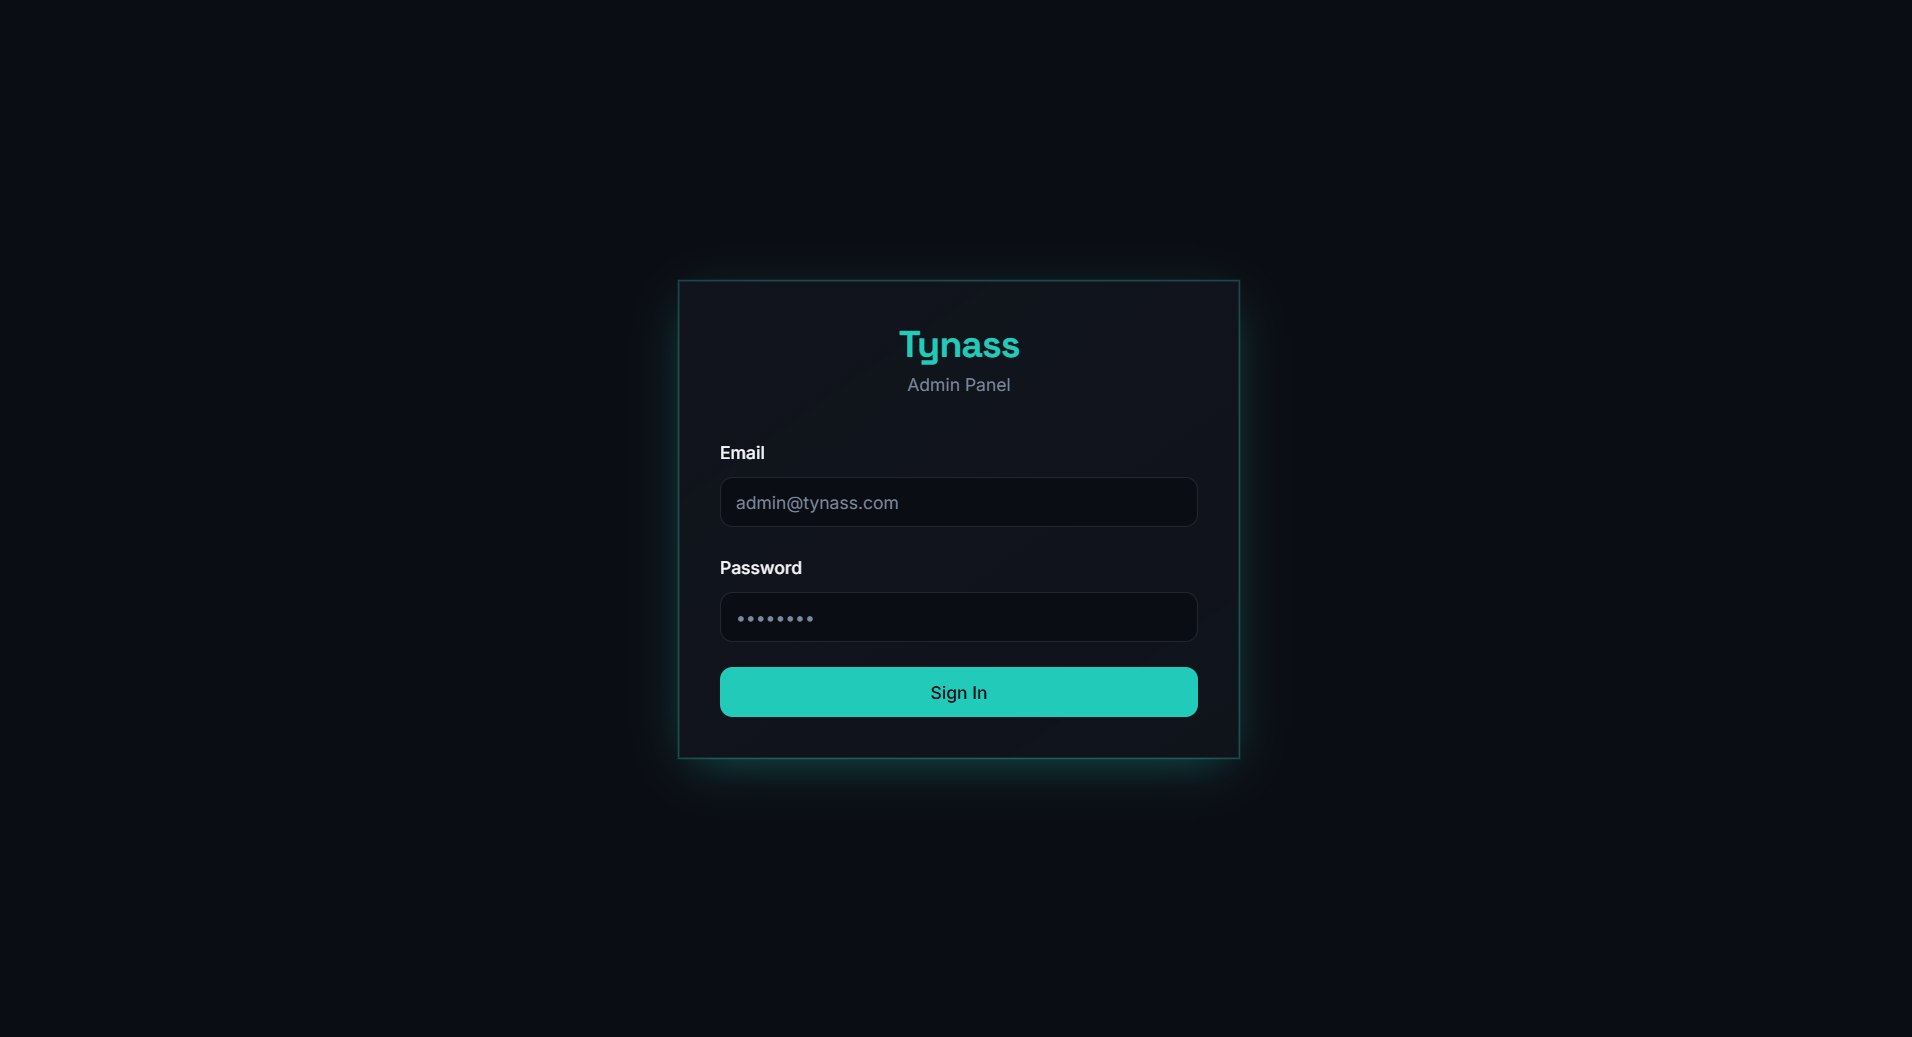
\includegraphics[width=0.8\textwidth]{../images/dashAdmin_login.png}
  \caption{Dashboard Admin --- page de connexion}
  \label{fig:dash_admin_login}
\end{figure}

\subsubsection{DashboardPage}

Page d'accueil affichant 4 KPIs calculés depuis le backend~: Total Companies, Total
Trainings, Sessions Played, Global Pass Rate. Affiche également les 5 entreprises
les plus actives et les 5 formations les plus jouées.

\begin{figure}[H]
  \centering
  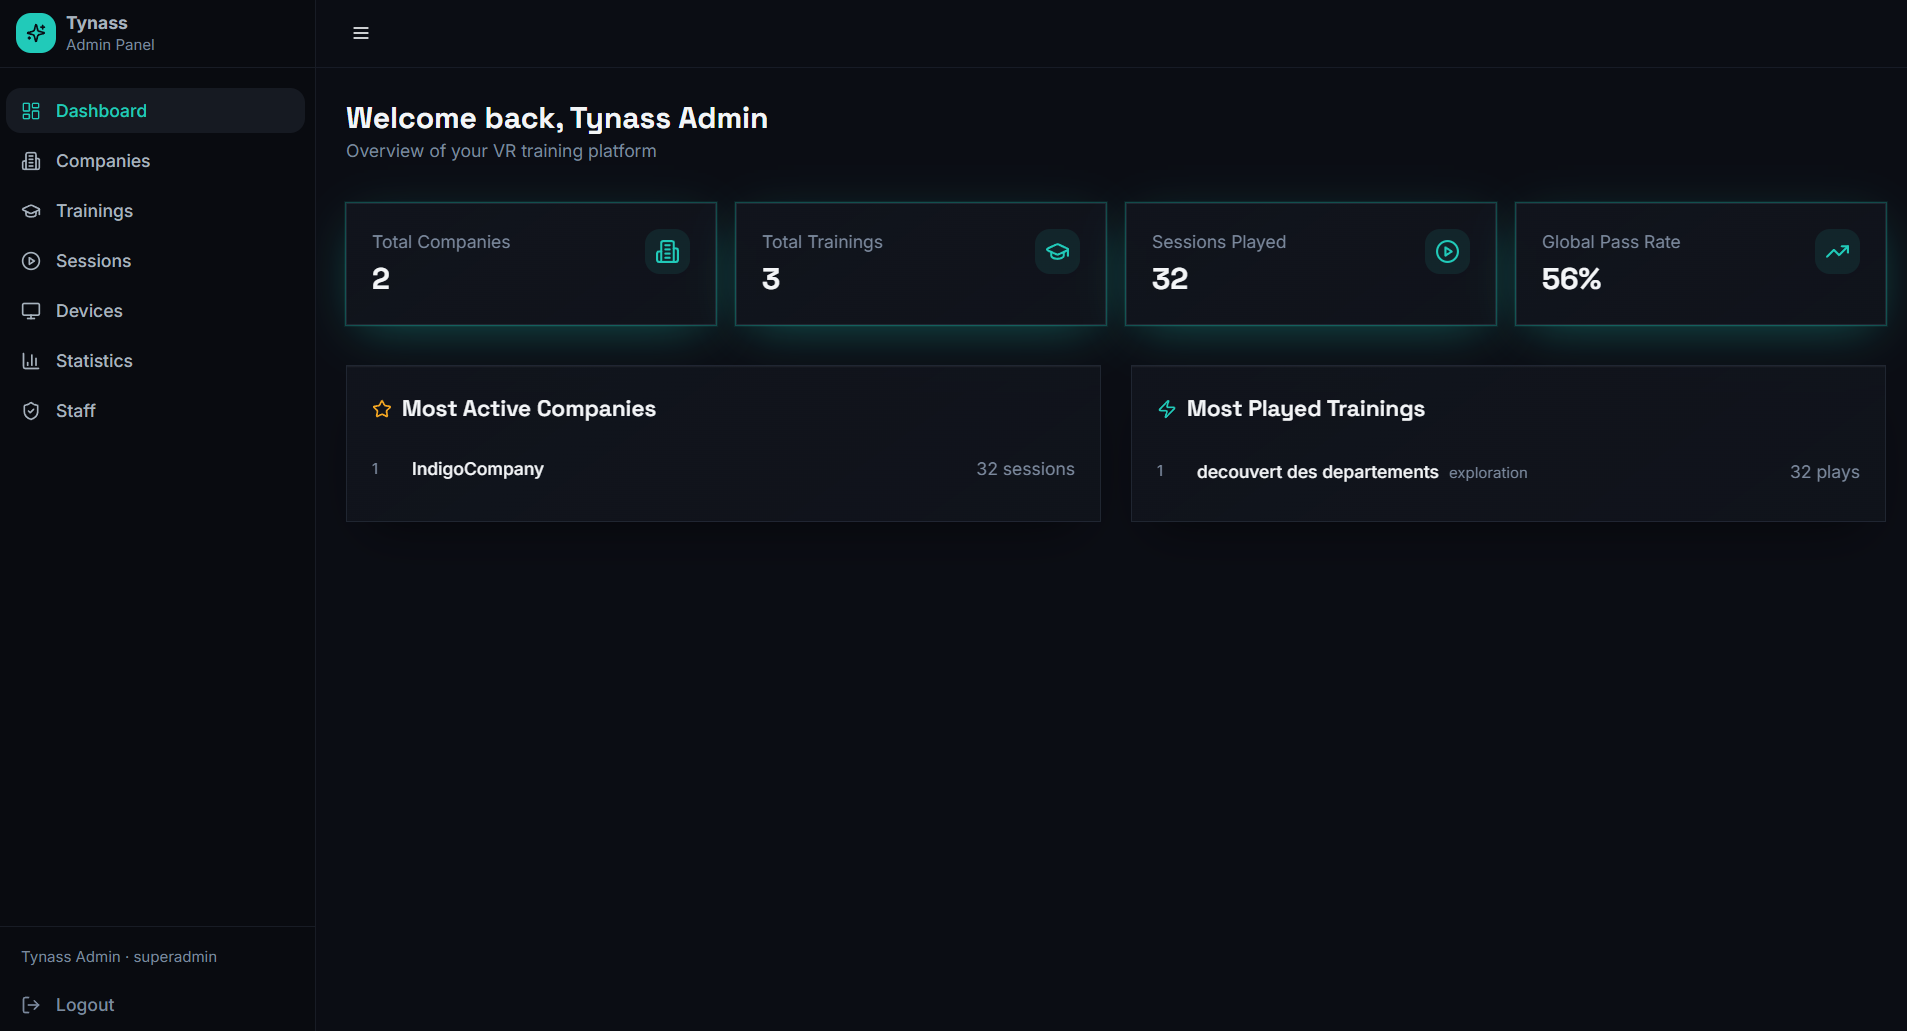
\includegraphics[width=\textwidth]{../images/dashAdmin_kpis.png}
  \caption{Dashboard Admin --- indicateurs clés (KPIs)}
  \label{fig:dash_admin_kpis}
\end{figure}

\subsubsection{CompaniesPage}

Gestion complète des entreprises clientes~: création, modification, suppression
(superadmin uniquement), activation/désactivation, et assignation des formations
via un dialog interactif.

\begin{figure}[H]
  \centering
  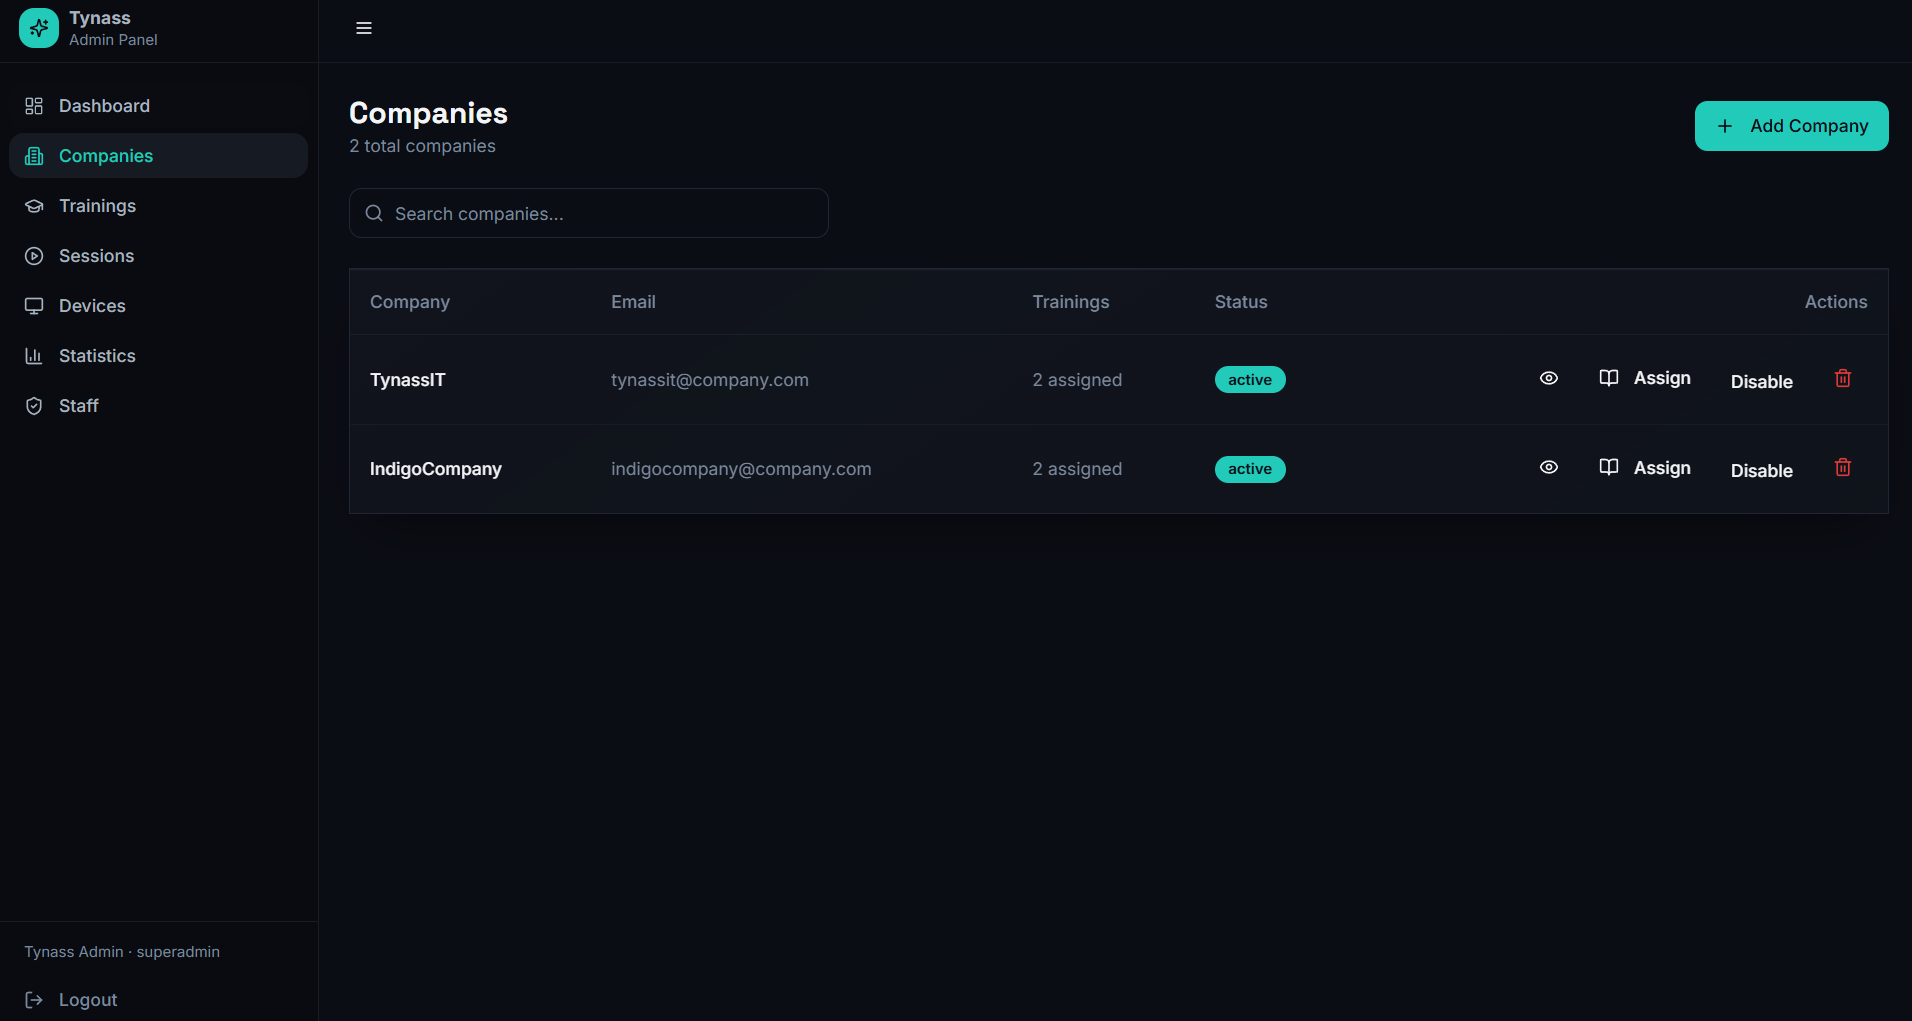
\includegraphics[width=\textwidth]{../images/dashAdmin_companies.png}
  \caption{Dashboard Admin --- gestion des entreprises}
  \label{fig:dash_admin_companies}
\end{figure}

\subsubsection{TrainingsPage}

Gestion du catalogue de formations VR. Le champ \texttt{sceneName} est crucial~: il
correspond exactement au nom de la scène Unity à charger via
\texttt{SceneManager.LoadScene(training.sceneName)}.

\begin{figure}[H]
  \centering
  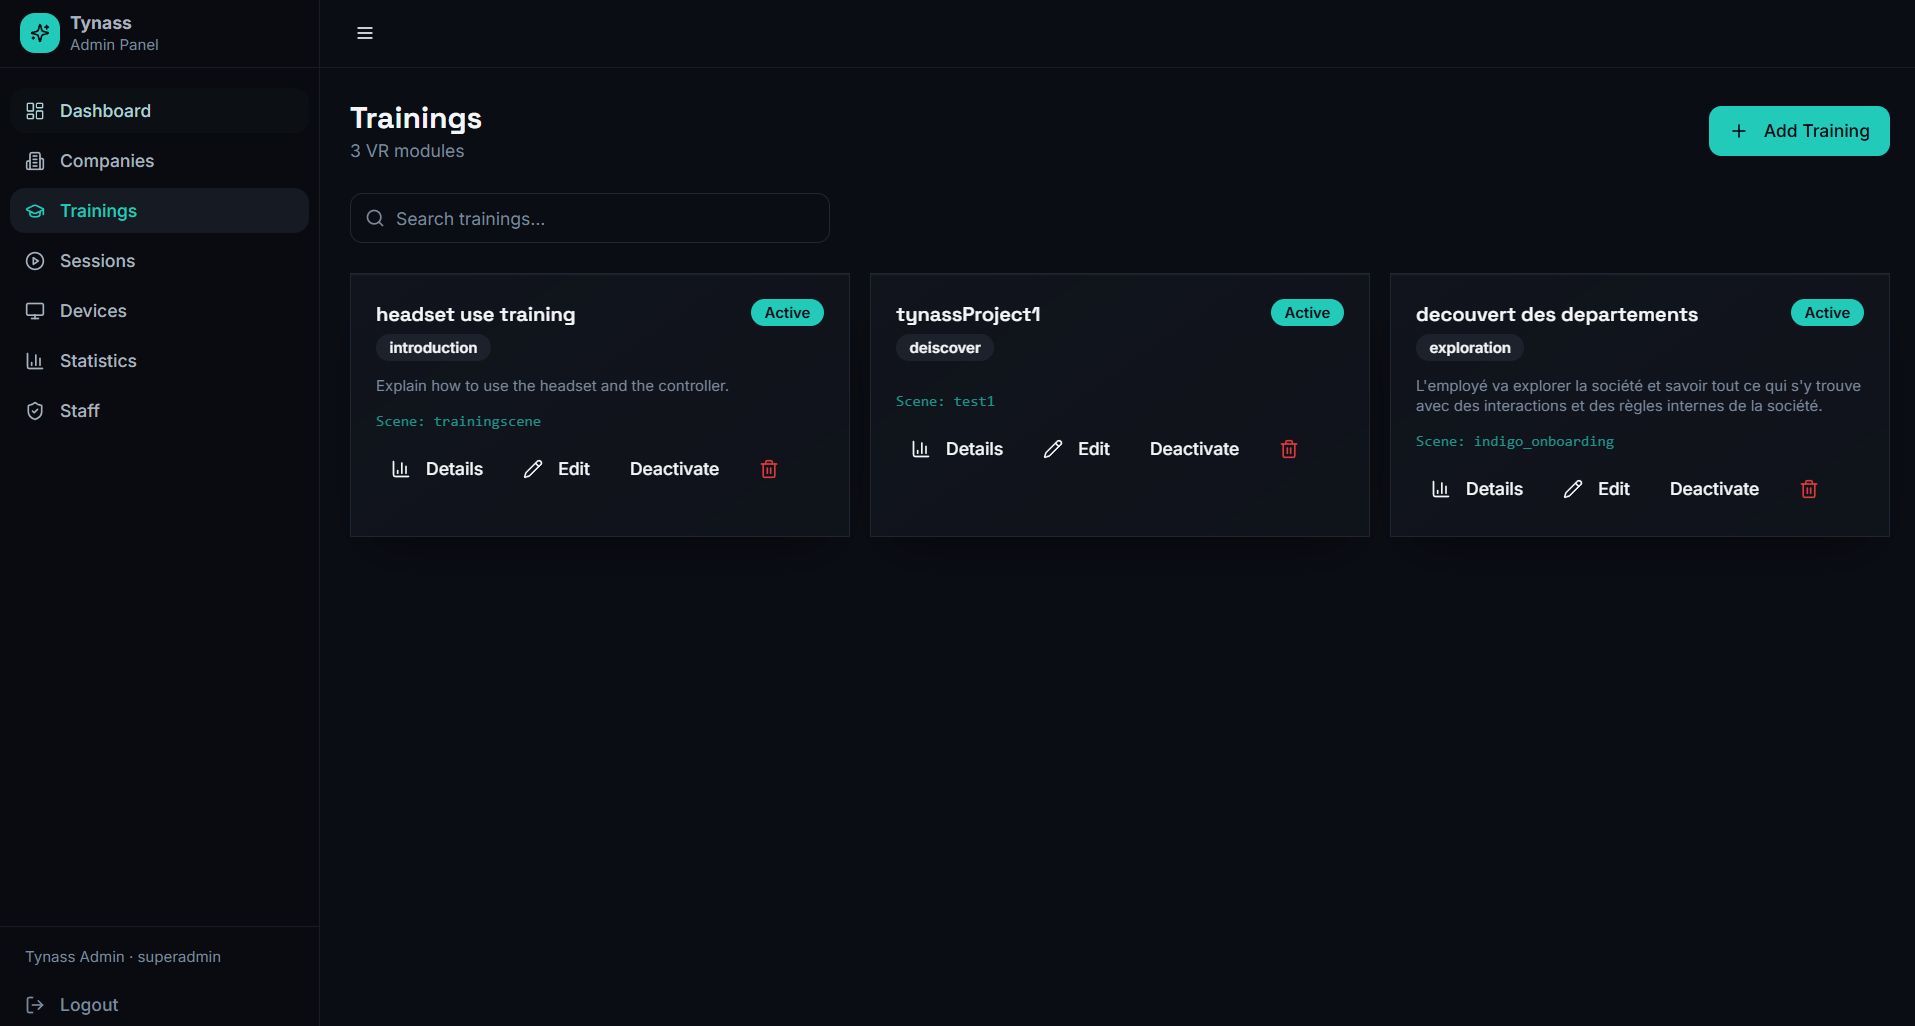
\includegraphics[width=\textwidth]{../images/dashAdmin_trainings.png}
  \caption{Dashboard Admin --- catalogue de formations et champ \texttt{sceneName}}
  \label{fig:dash_admin_trainings}
\end{figure}

\subsubsection{DevicesPage}

Activation et révocation des casques Meta Quest~3. L'admin saisit le code 6 chiffres
affiché sur le casque, sélectionne l'entreprise et confirme l'activation.

\begin{figure}[H]
  \centering
  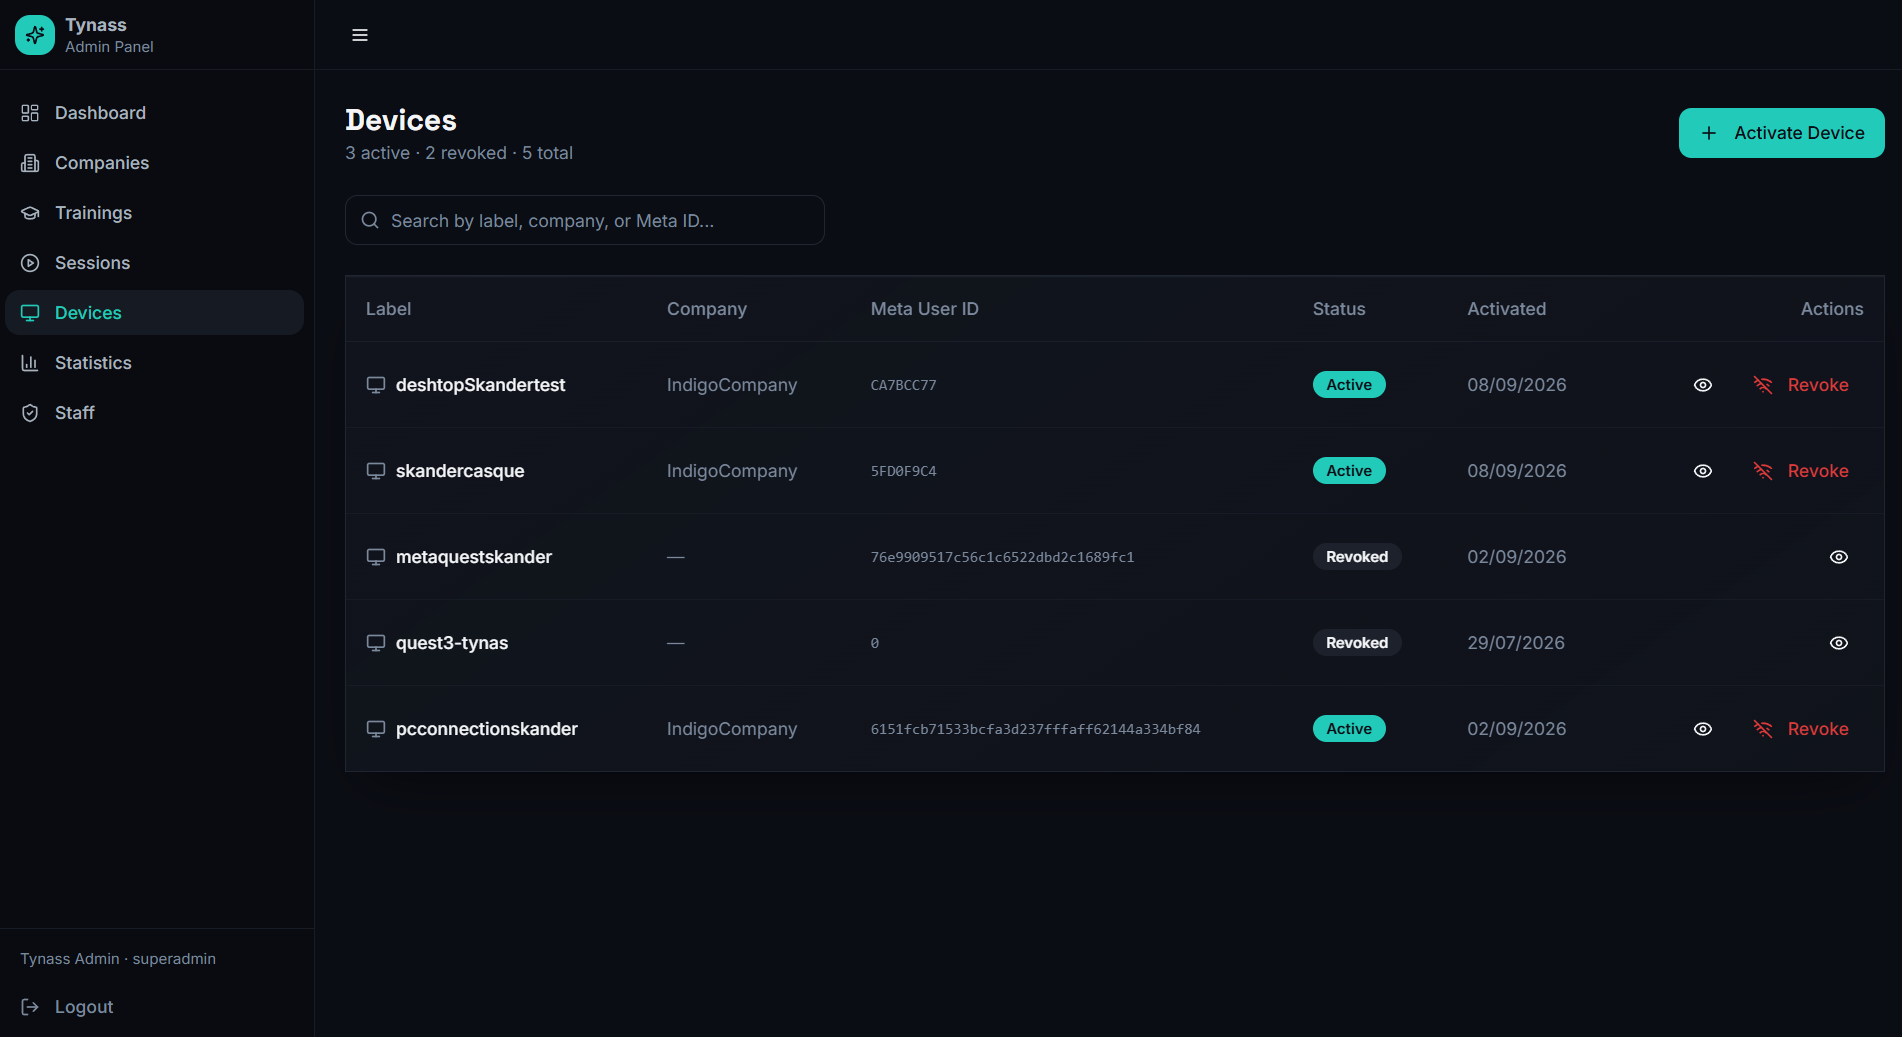
\includegraphics[width=\textwidth]{../images/dashAdmin_devices.png}
  \caption{Dashboard Admin --- activation d'un casque}
  \label{fig:dash_admin_devices}
\end{figure}

\subsubsection{SessionsPage}

Historique de toutes les sessions avec filtres multi-critères~: \texttt{companyFilter},
\texttt{trainingFilter}, \texttt{dateFrom}, \texttt{dateTo}. Le filtrage est effectué
côté client (JavaScript) sur le tableau complet retourné par l'API.

\begin{figure}[H]
  \centering
  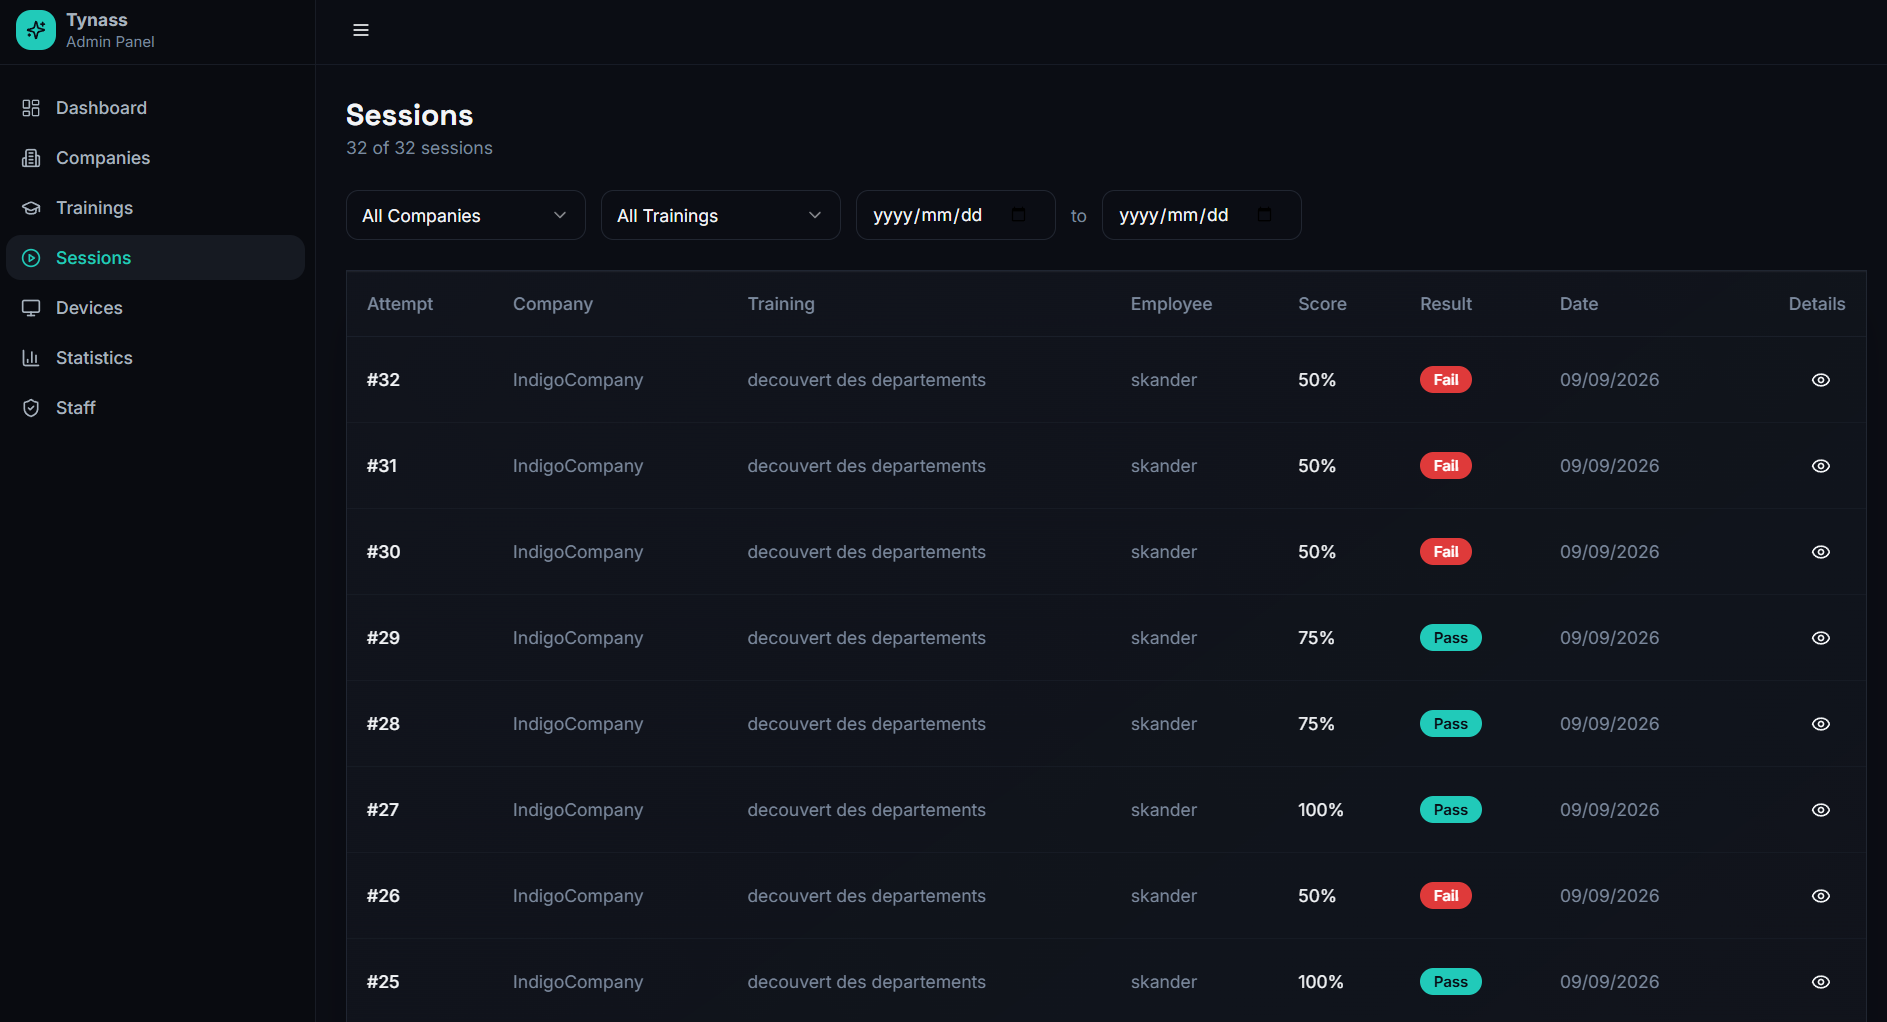
\includegraphics[width=\textwidth]{../images/dashAdmin_sessions.png}
  \caption{Dashboard Admin --- historique des sessions et filtres}
  \label{fig:dash_admin_sessions}
\end{figure}

\subsubsection{StatisticsPage}

Visualisation des statistiques agrégées par formation et par entreprise, calculées
via les pipelines d'agrégation MongoDB.

\begin{figure}[H]
  \centering
  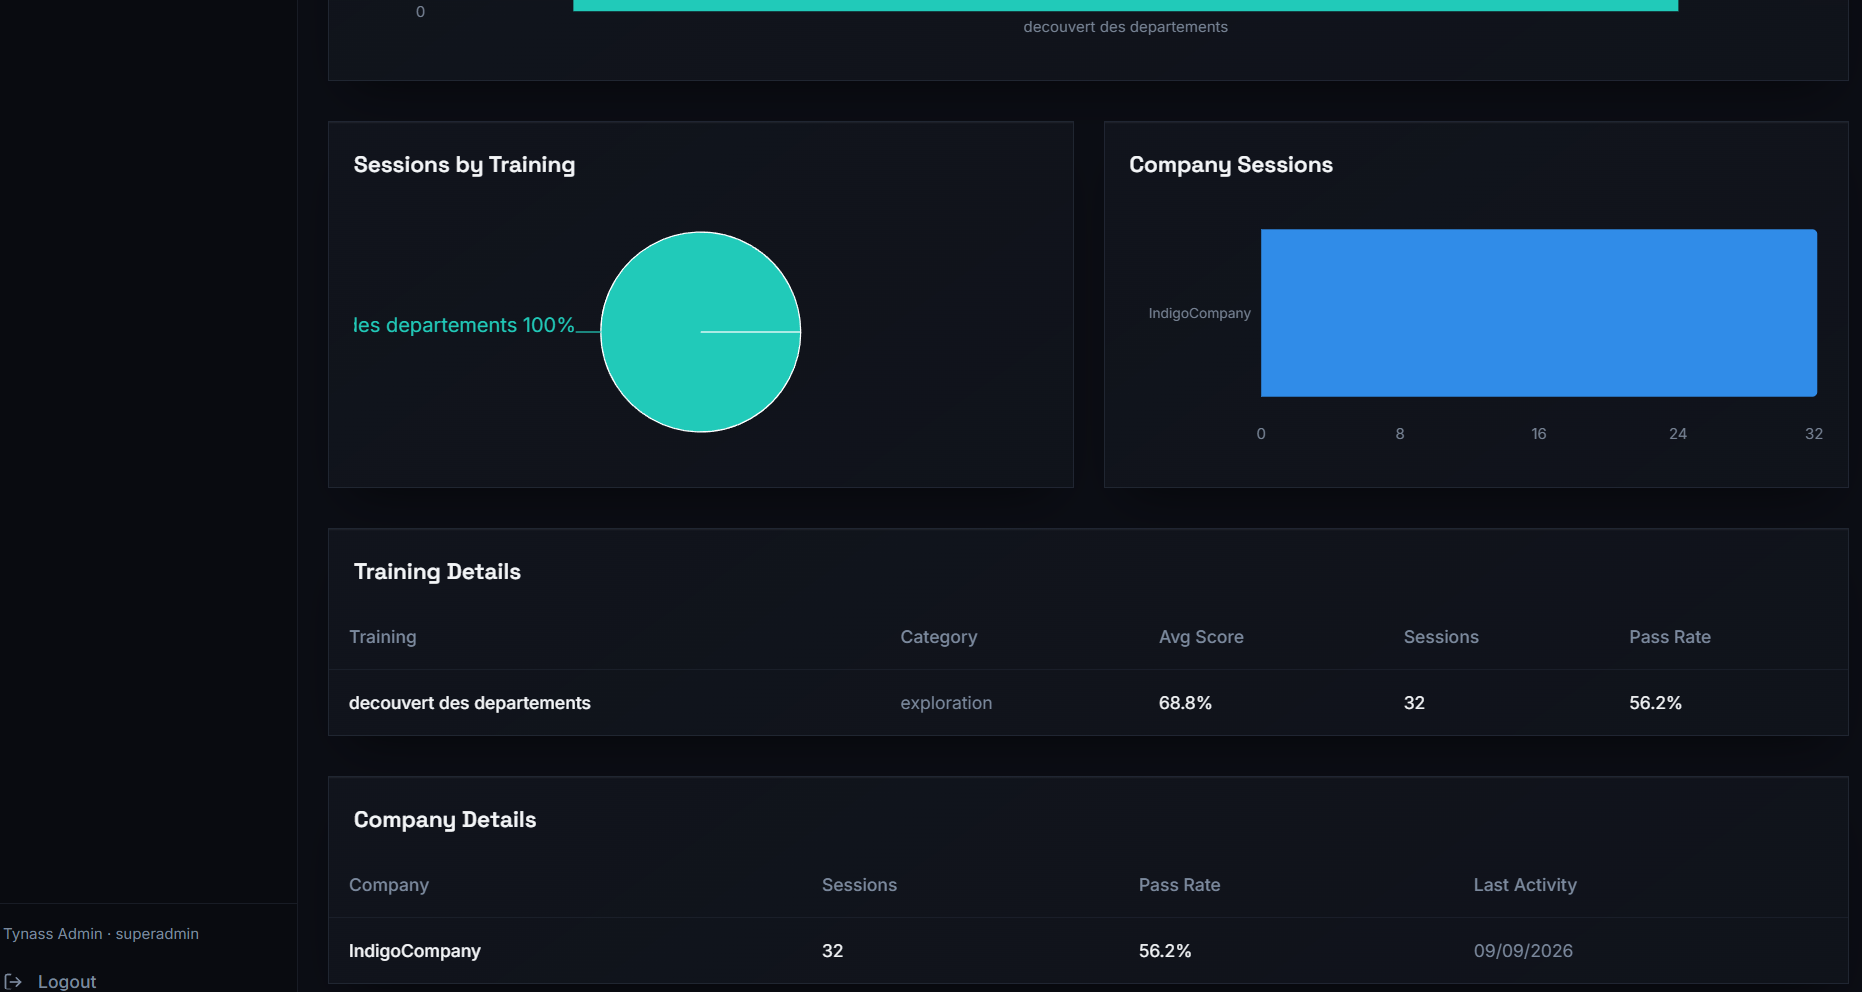
\includegraphics[width=\textwidth]{../images/dashAdmin_stats.png}
  \caption{Dashboard Admin --- statistiques agrégées}
  \label{fig:dash_admin_stats}
\end{figure}

\subsection{Dashboard Company --- Pages implémentées}

Le dashboard Company regroupe les pages permettant à l'entreprise de gérer ses employés
et de suivre leurs sessions.

\subsubsection{EmployeesPage}

Page centrale du dashboard Company~: CRUD complet des employés, affichage de
l'accessCode (lecture seule après création), saisie du PIN lors de la création, et
consultation des milestones de chaque employé.

\begin{figure}[H]
  \centering
  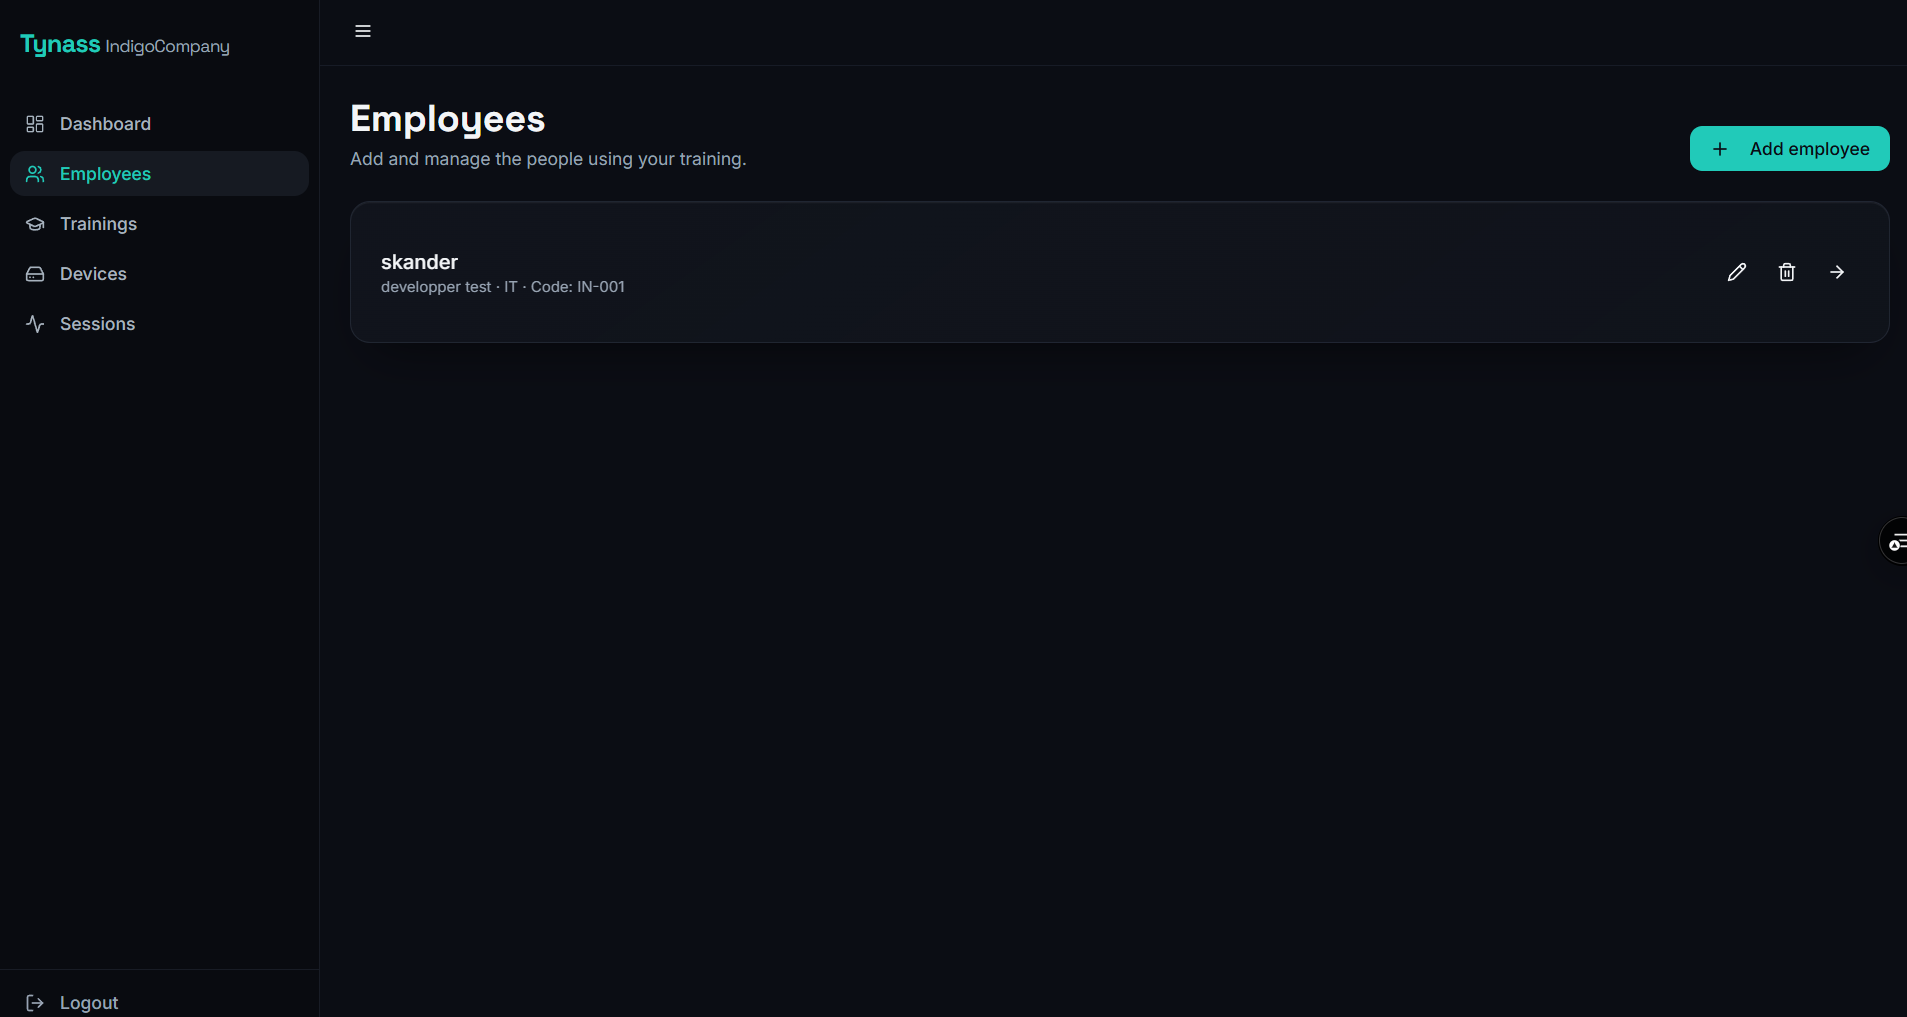
\includegraphics[width=\textwidth]{../images/dashCompany_employees.png}
  \caption{Dashboard Company --- gestion des employés}
  \label{fig:dash_company_employees}
\end{figure}

\subsubsection{SessionsPage Company}

Historique des sessions avec pagination frontend (PAGE\_SIZE = 20 sessions par page),
filtrage par employé ou par formation.

\begin{figure}[H]
  \centering
  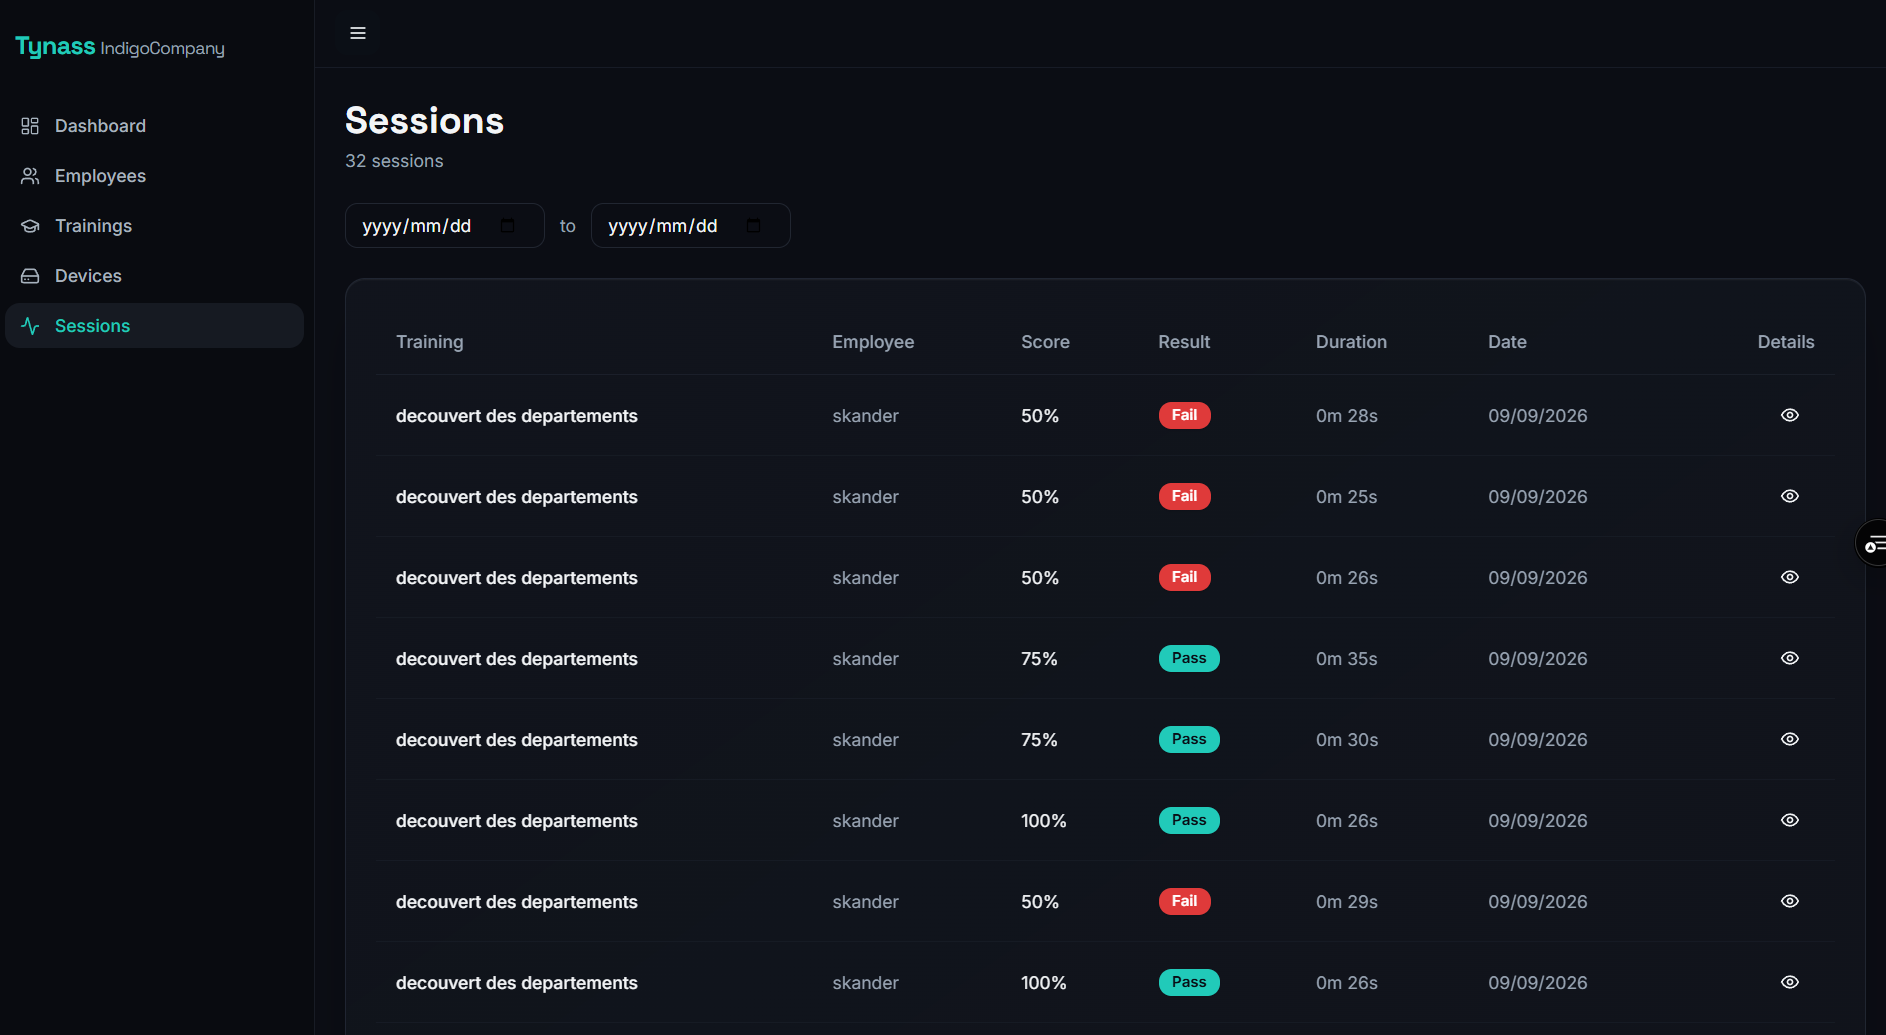
\includegraphics[width=\textwidth]{../images/dashCompany_sessions.png}
  \caption{Dashboard Company --- historique des sessions}
  \label{fig:dash_company_sessions}
\end{figure}

\section{Difficultés et solutions}

\begin{table}[H]
  \centering
  \begin{tabularx}{\textwidth}{lXX}
    \toprule
    \textbf{Défi} & \textbf{Problème} & \textbf{Solution} \\
    \midrule
    Migration router & TanStack Start (SSR) bloquait les appels
                       fetch côté client en production. &
                       Migration vers React Router v6~: routage
                       100\% côté client, sans SSR. \\
    \midrule
    Tailwind v4 & Shadcn UI incompatible avec Tailwind v4
                  (classes manquantes, styles cassés). &
                  Migration vers Tailwind v3, stable et
                  pleinement compatible avec Shadcn. \\
    \midrule
    Pattern \texttt{?? data} & Le backend enveloppe les réponses~:
                               \texttt{\{companies: [...]\}} au lieu de
                               \texttt{[...]} directement. &
                               Pattern \texttt{data.companies ?? data}
                               dans chaque appel API pour
                               rétrocompatibilité. \\
    \midrule
    Tri statistiques & Le champ \texttt{sessionsPlayed} dans les
                       mock-data ne correspondait pas au champ
                       \texttt{totalSessions} retourné par le backend. &
                       Correction du tri~: utilisation de
                       \texttt{totalSessions} (champ backend réel). \\
    \midrule
    CORS & Le dashboard (localhost:8080) était bloqué
           par le backend sans configuration CORS. &
           Ajout du middleware cors() avant toutes les
           routes, avec origines explicites. \\
    \bottomrule
  \end{tabularx}
  \caption{Difficultés rencontrées et solutions --- Itération~2}
  \label{tab:dificultes_s2}
\end{table}

\section{Évaluation de l'itération~2}

\begin{table}[H]
  \centering
  \begin{tabular}{ll}
    \toprule
    \textbf{Élément validé} & \textbf{Statut} \\
    \midrule
    Pages du dashboard Admin livrées   & 7 / 7 \\
    Pages du dashboard Company livrées & 6 / 6 \\
    Connexion des dashboards à l'API REST & Fonctionnel \\
    Déploiement en production sur Vercel & Fonctionnel \\
    \bottomrule
  \end{tabular}
  \caption{Validation fonctionnelle --- Itération~2}
  \label{tab:eval_s2}
\end{table}

Les deux dashboards sont déployés en production sur Vercel, comme le montre
la figure~\ref{fig:dashboards_vercel}.

\begin{figure}[H]
  \centering
  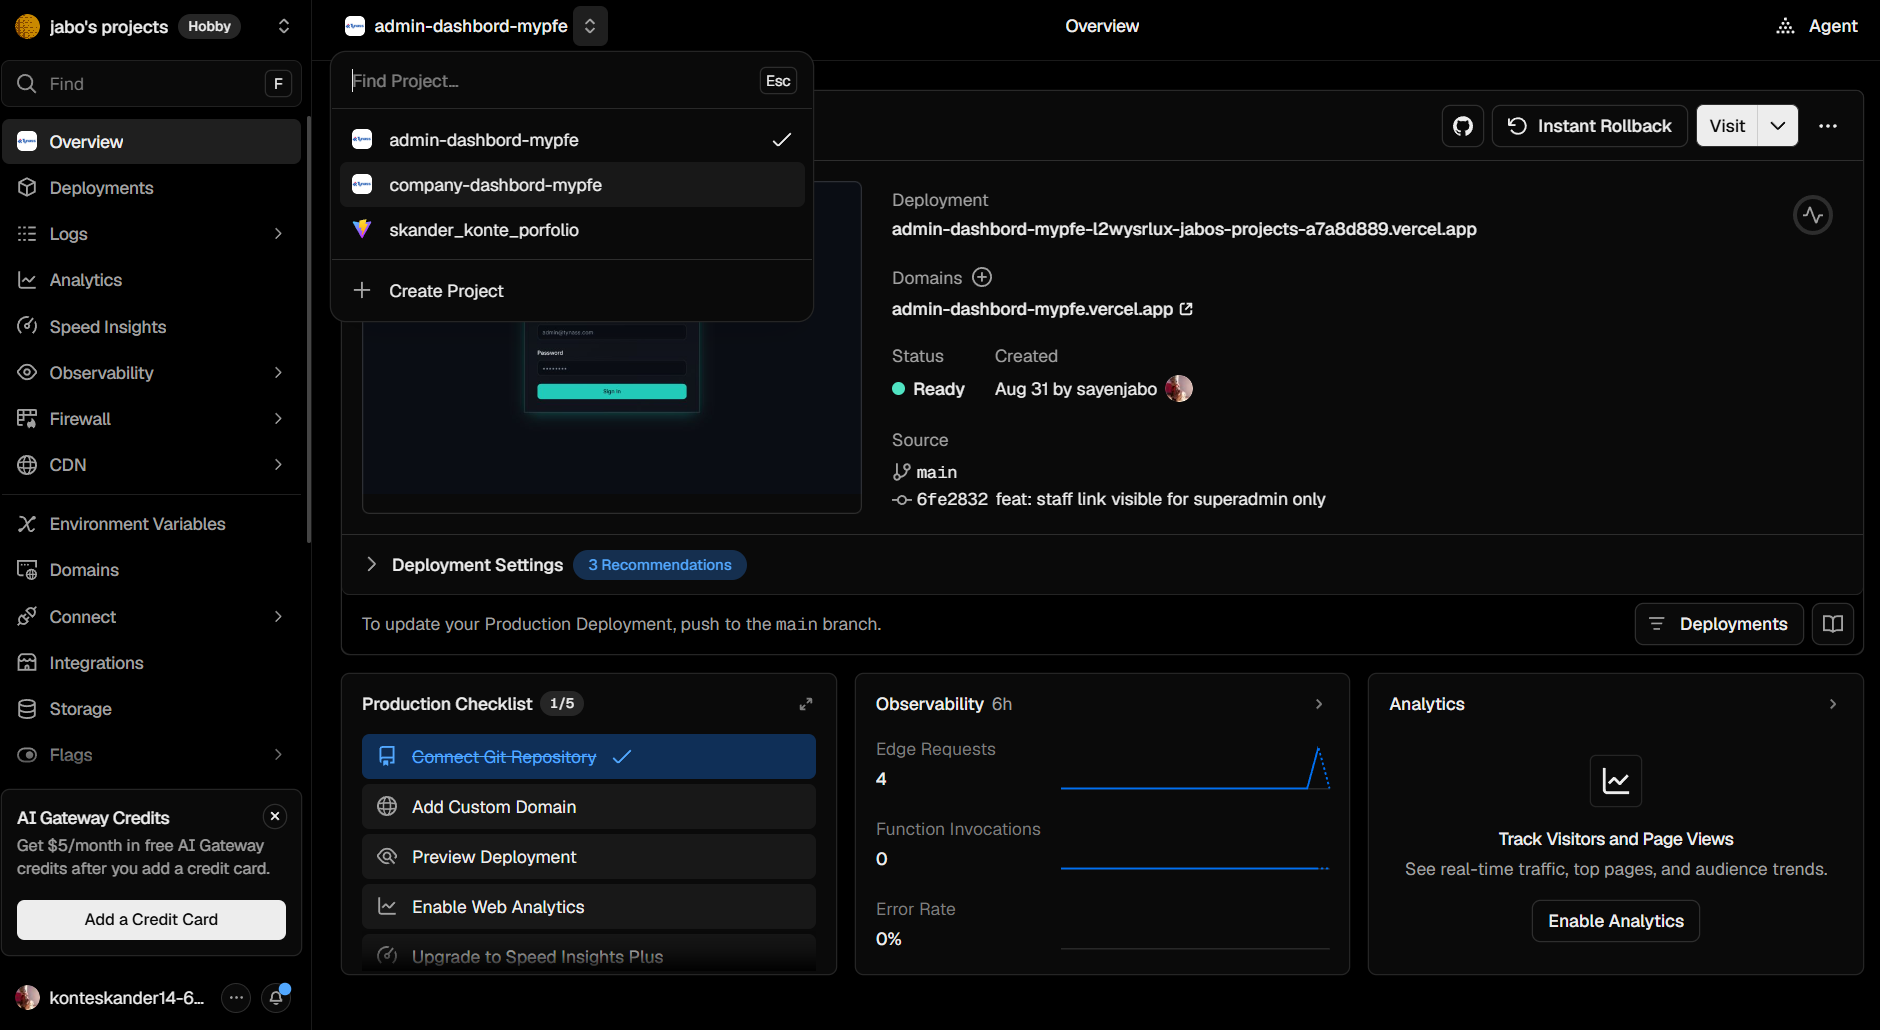
\includegraphics[width=\textwidth]{../images/dashboards_vercel.png}
  \caption{Les deux dashboards déployés en production sur Vercel}
  \label{fig:dashboards_vercel}
\end{figure}

\section{Conclusion}

Cette deuxième itération a livré les deux dashboards web de \tynassit{}, déployés sur Vercel~:
\texttt{admin-dashbord-mypfe.vercel.app} et \texttt{company-dashbord-mypfe.vercel.app}.
Les 8 user stories couvertes ont toutes été livrées. Le chapitre suivant
présente le développement de l'application VR.
